\section{Semantic Segmentation}
\begin{frame}{}
    \LARGE Image Segmentation: \textbf{Semantic Segmentation}
\end{frame}

\begin{frame}[allowframebreaks]{Semantic Segmentation}
    \begin{figure}
        \centering
        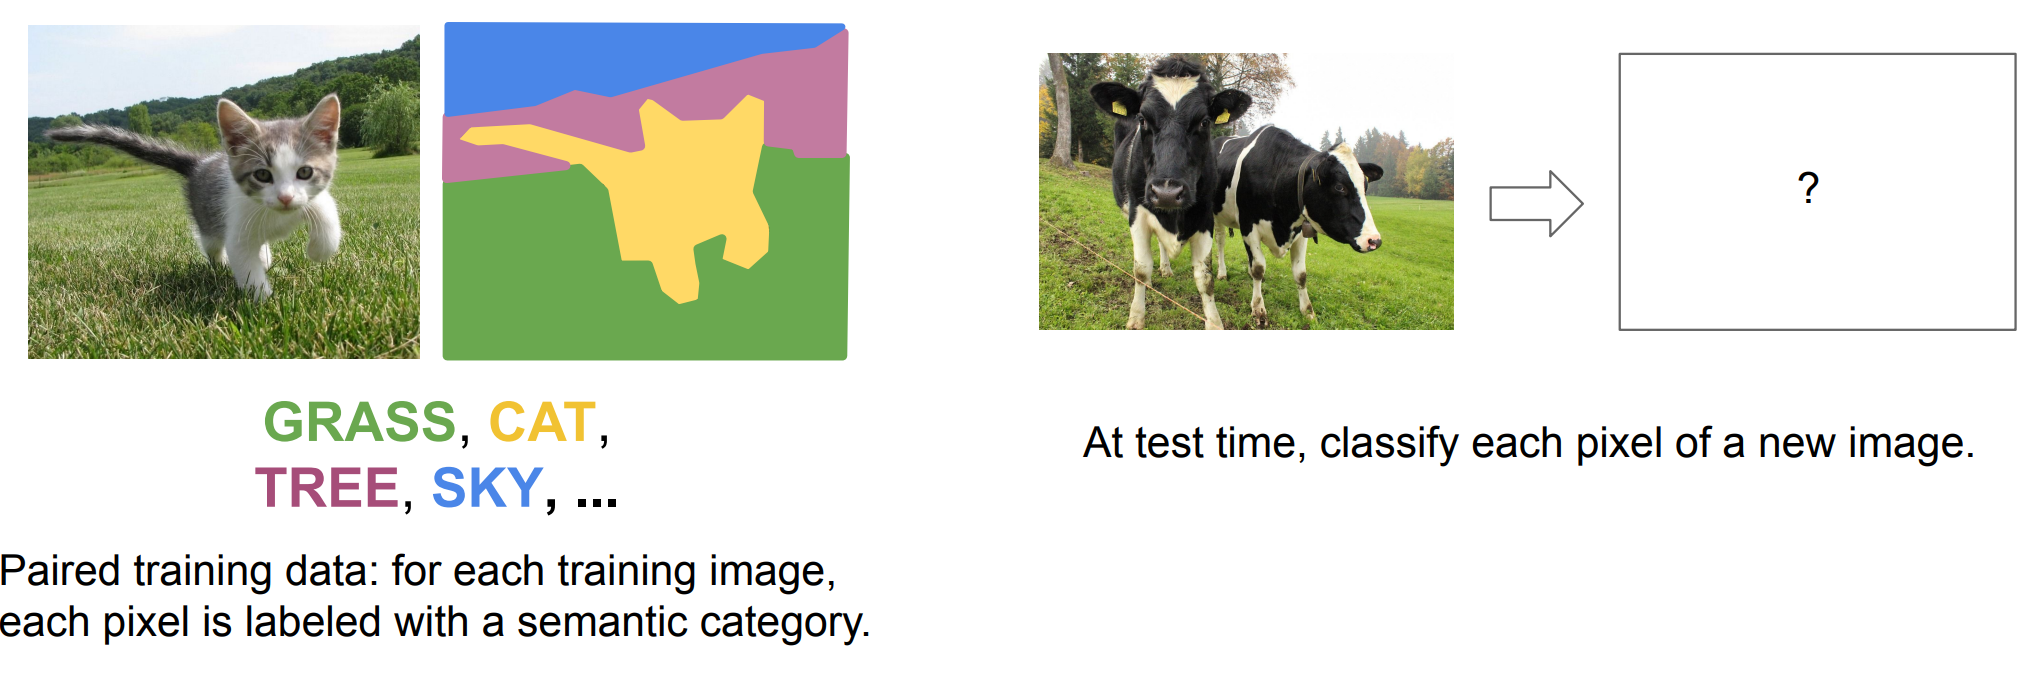
\includegraphics[width=1.0\textwidth,height=1.0\textheight,keepaspectratio]{images/segmentation/sem_1.png}
    \end{figure}
    
\framebreak

    \begin{figure}
        \centering
        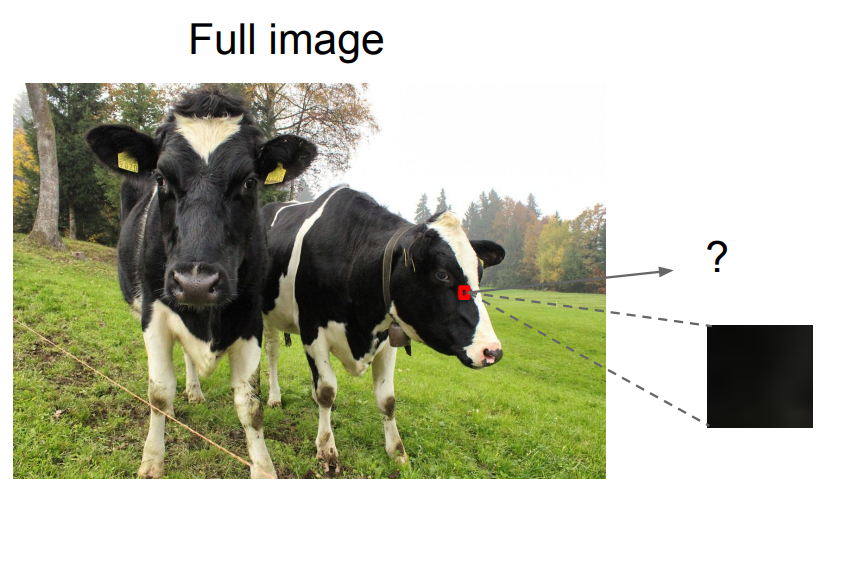
\includegraphics[width=1.0\textwidth,height=0.7\textheight,keepaspectratio]{images/segmentation/sem_2.png}
    \end{figure}
    \pause

    \begin{itemize}
        \item Impossible to classify without context
        \item How do we include context?
    \end{itemize}
\end{frame}

\subsection{Sliding Window}

\begin{frame}[allowframebreaks]{Semantic Segmentation Idea: Sliding Window}
    \begin{figure}
        \centering
        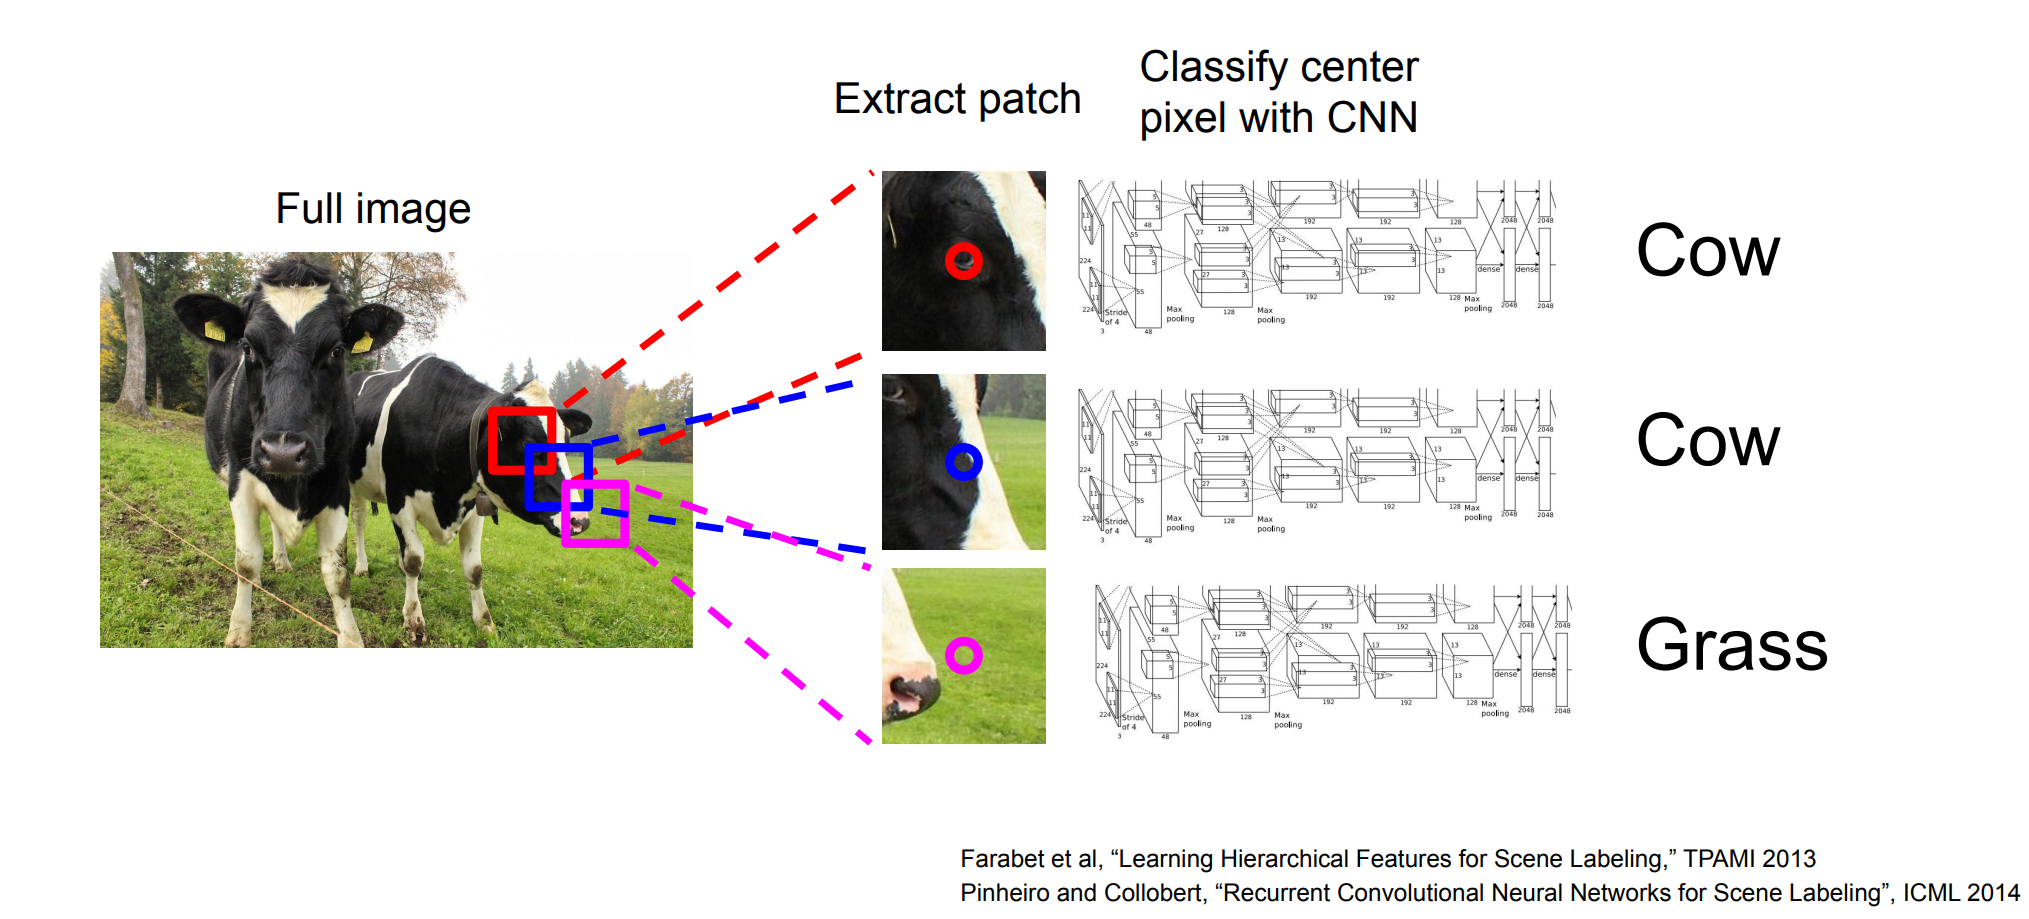
\includegraphics[width=1.0\textwidth,height=1.0\textheight,keepaspectratio]{images/segmentation/sem_3.png}
    \end{figure}

\framebreak

    \begin{figure}
        \centering
        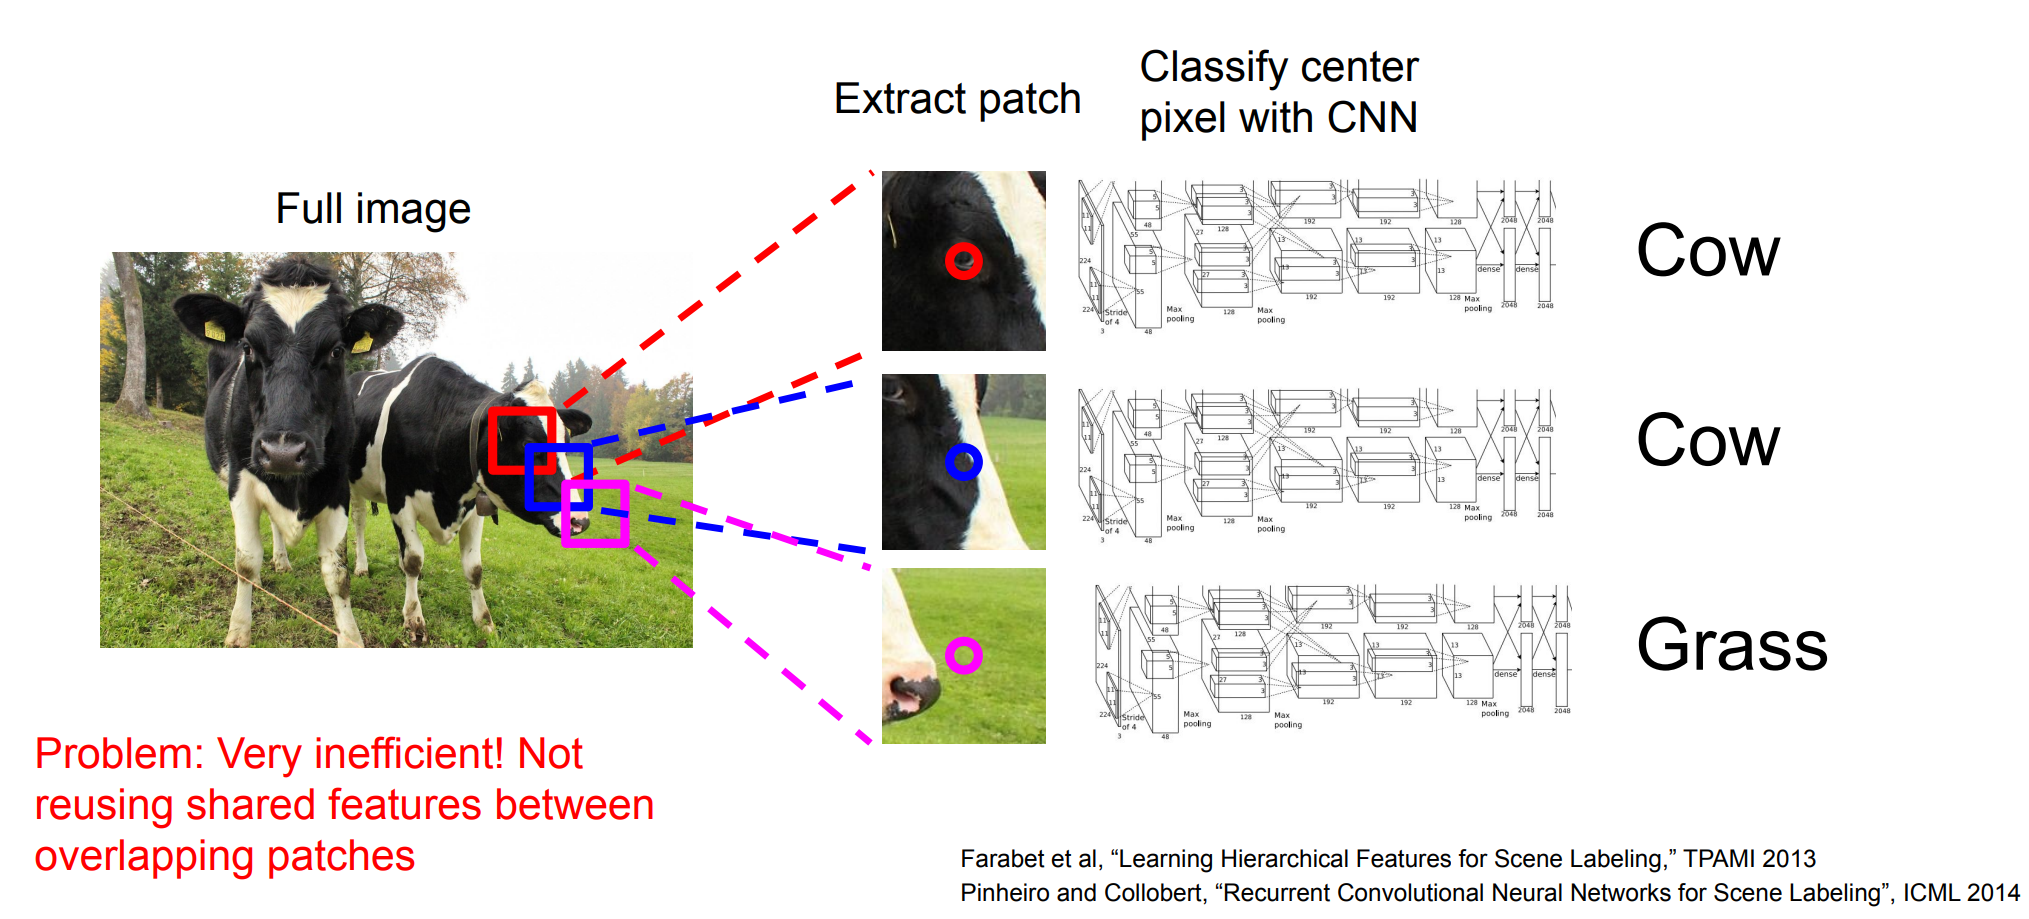
\includegraphics[width=1.0\textwidth,height=1.0\textheight,keepaspectratio]{images/segmentation/sem_4.png}
    \end{figure}
    
\end{frame}
\subsection{Convolution}

\begin{frame}[allowframebreaks]{Semantic Segmentation Idea: Convolution}
\begin{figure}
\centering
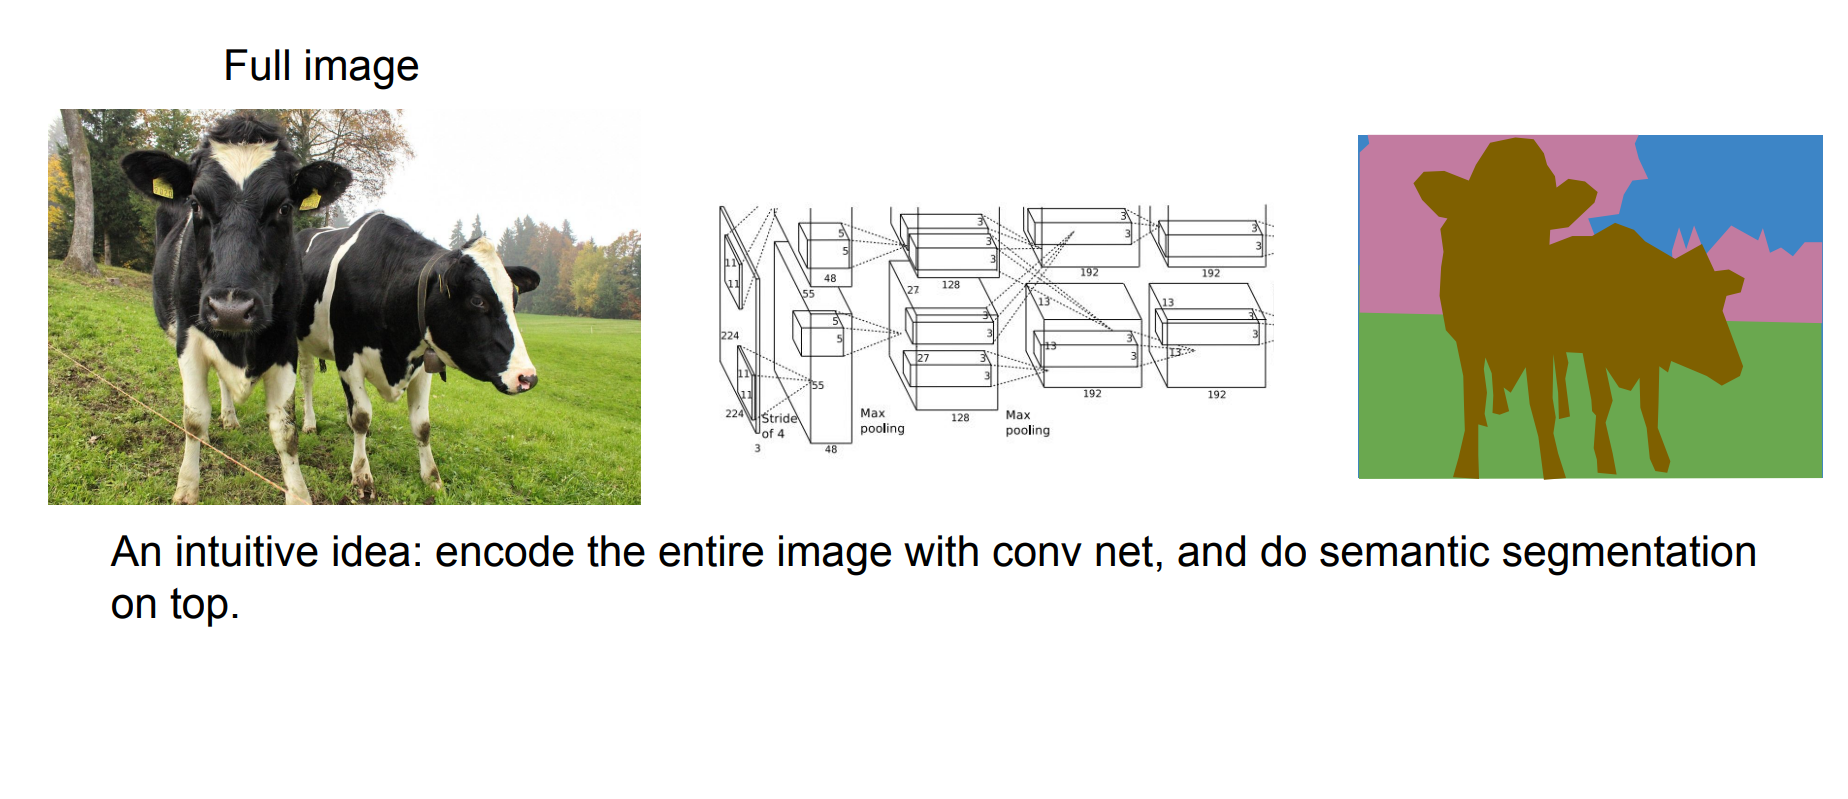
\includegraphics[width=1.0\textwidth,height=1.0\textheight,keepaspectratio]{images/segmentation/sem_5.png}
\end{figure}

\framebreak

\begin{figure}
\centering
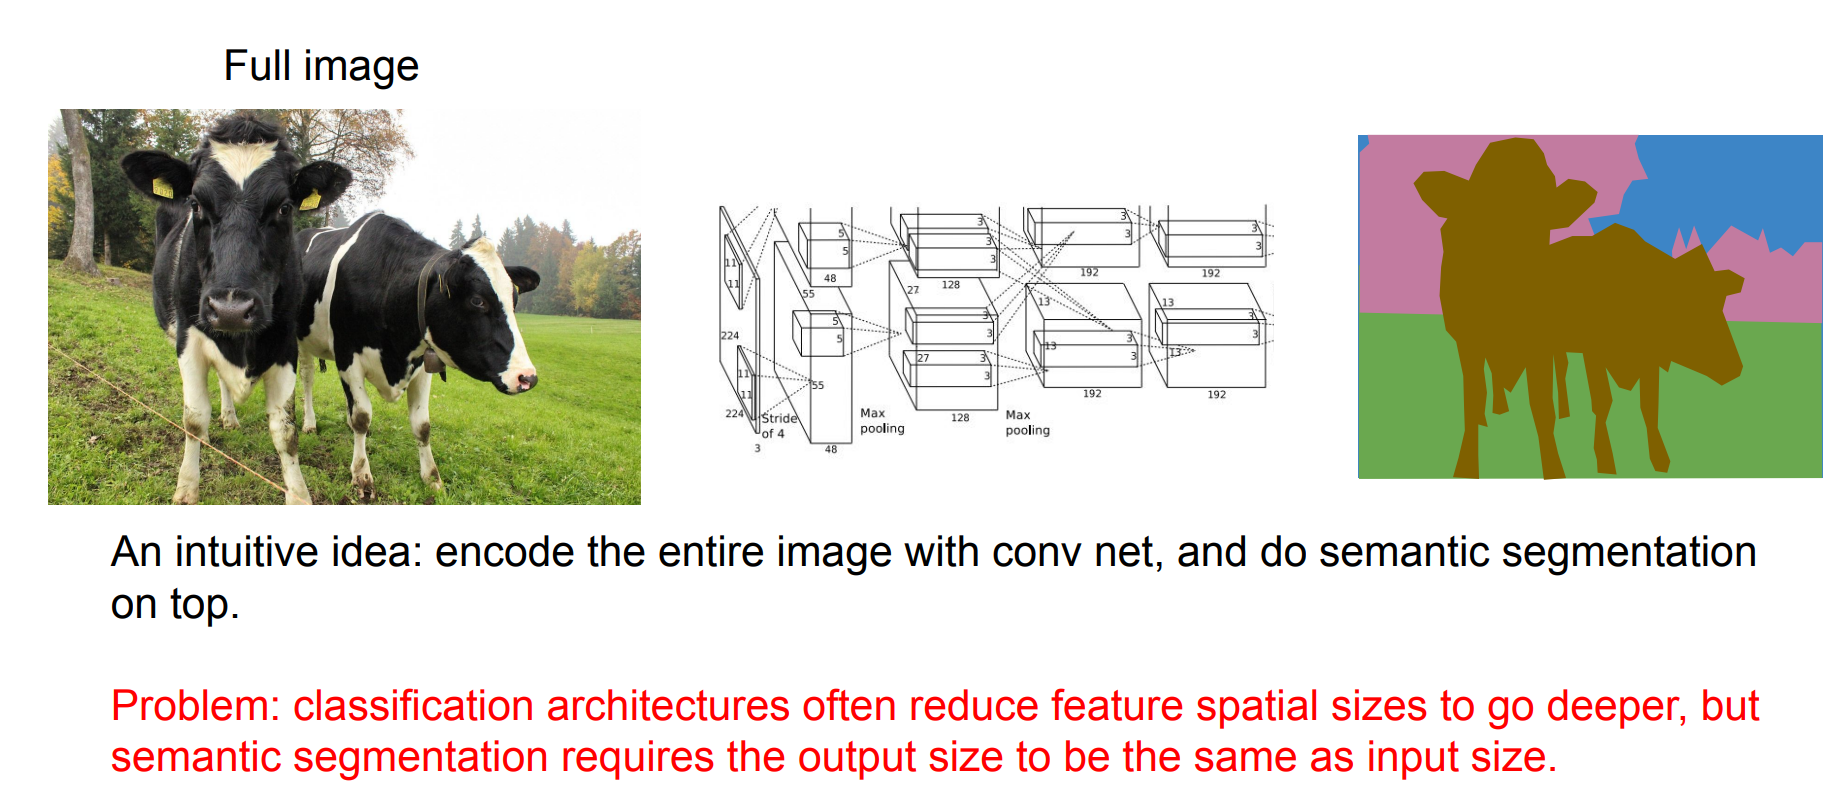
\includegraphics[width=1.0\textwidth,height=1.0\textheight,keepaspectratio]{images/segmentation/sem_6.png}
\end{figure}
    
\end{frame}

\begin{frame}[allowframebreaks]{Semantic Segmentation Idea: Fully Convolutional}
\begin{figure}
\centering
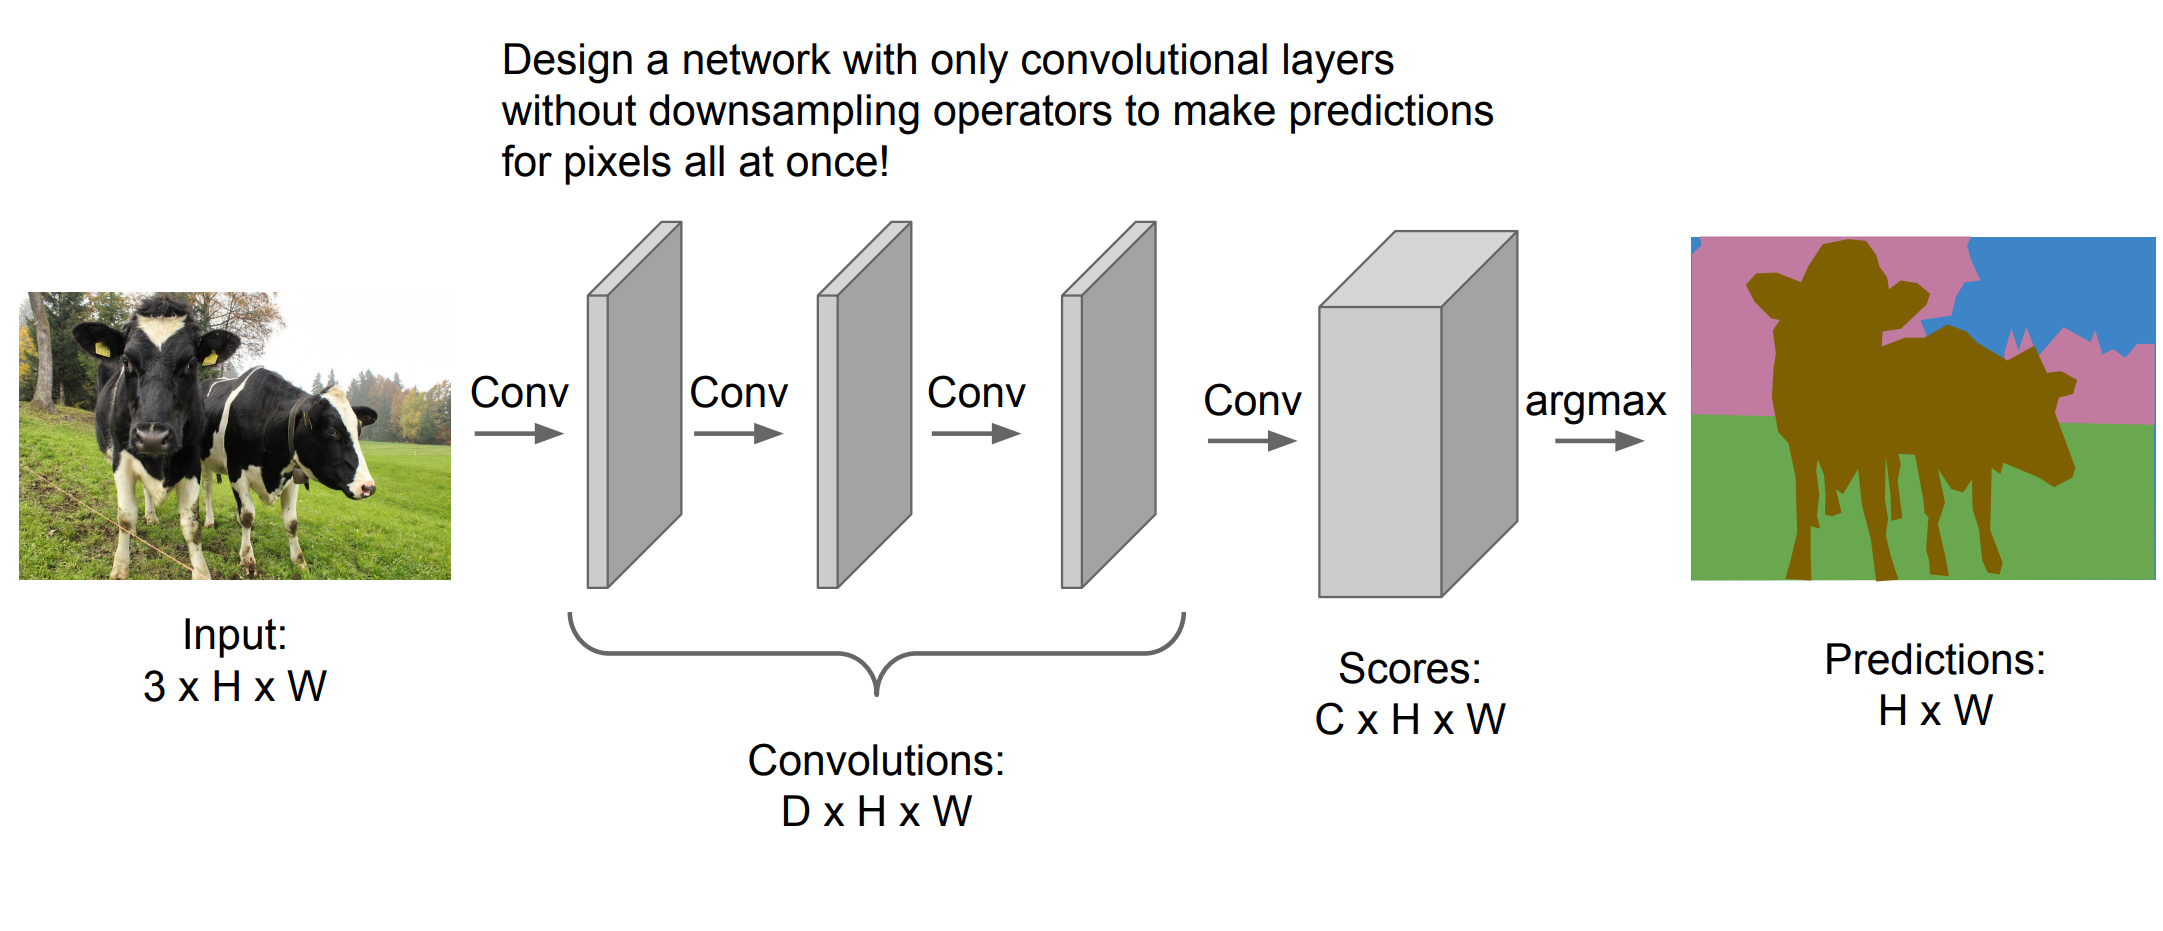
\includegraphics[width=1.0\textwidth,height=1.0\textheight,keepaspectratio]{images/segmentation/sem_7.png}
\end{figure}

\framebreak

\begin{figure}
\centering
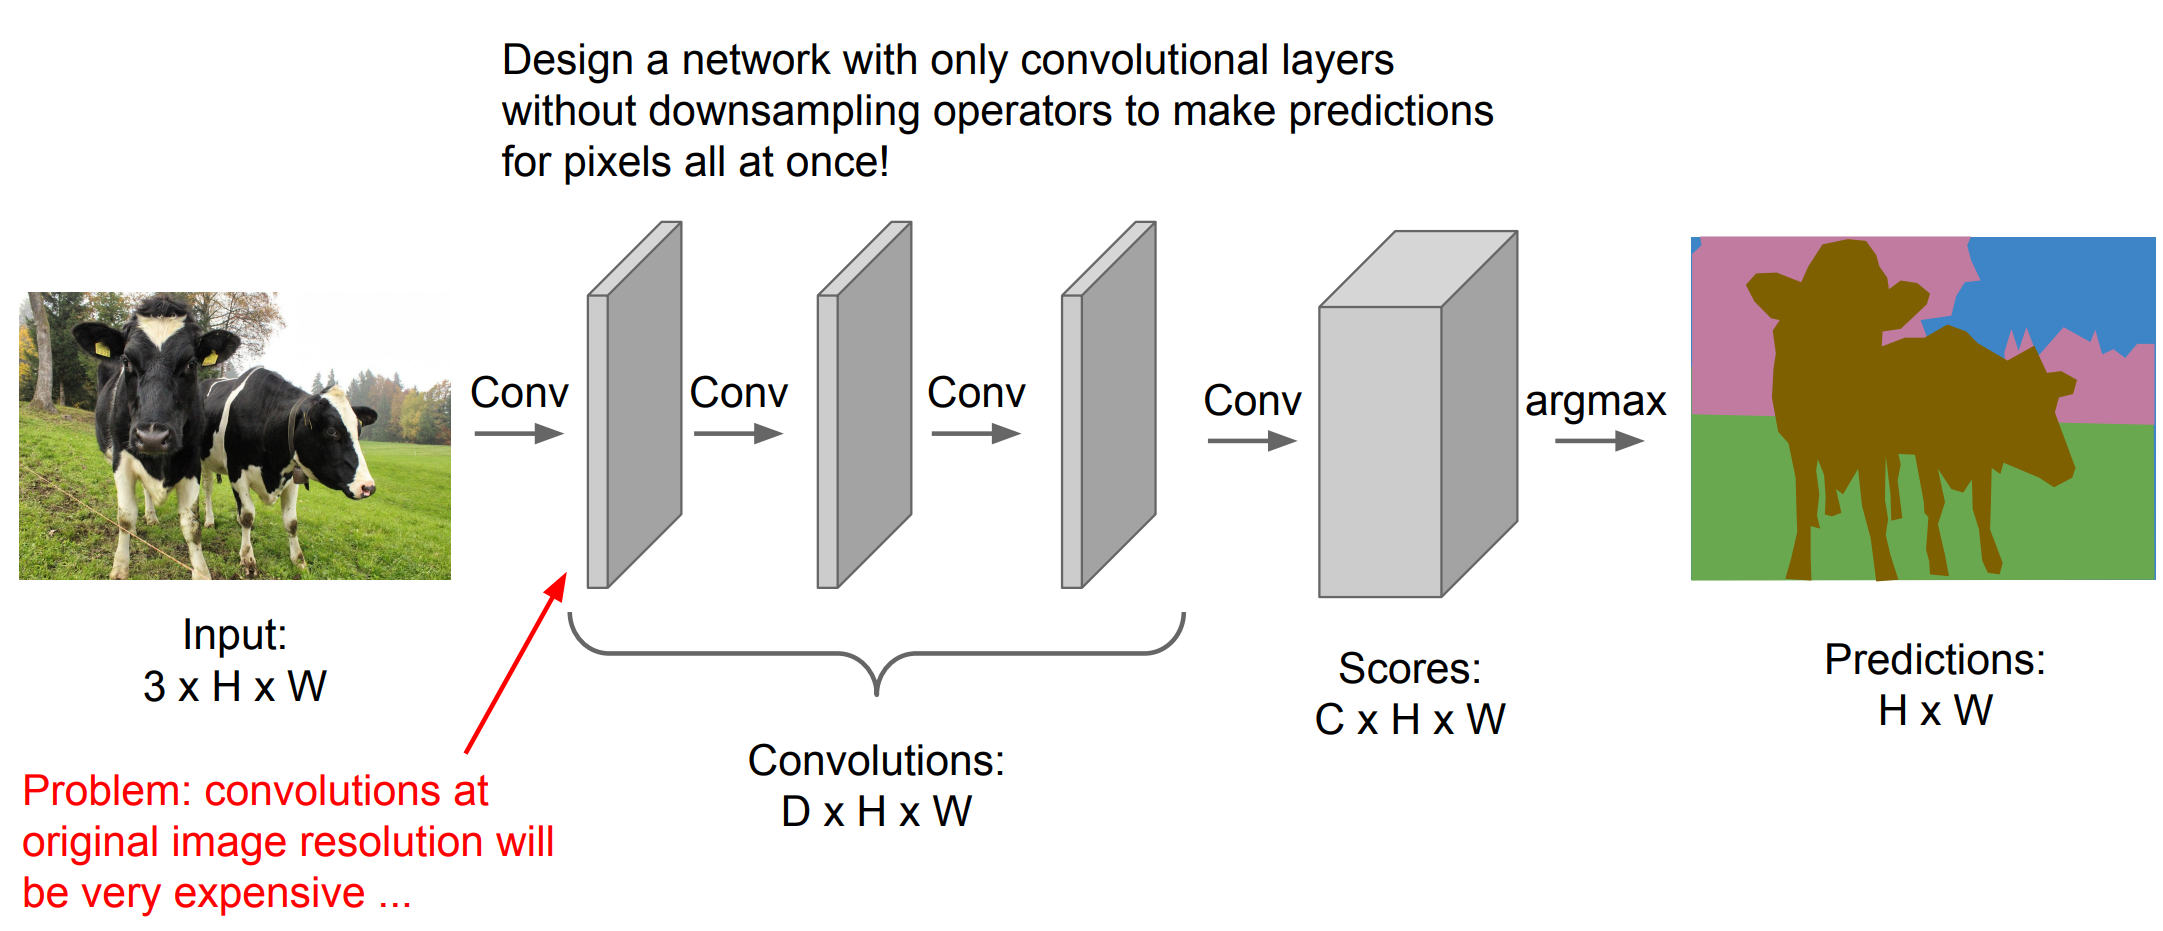
\includegraphics[width=1.0\textwidth,height=1.0\textheight,keepaspectratio]{images/segmentation/sem_8.png}
\end{figure}

\framebreak

\begin{figure}
\centering
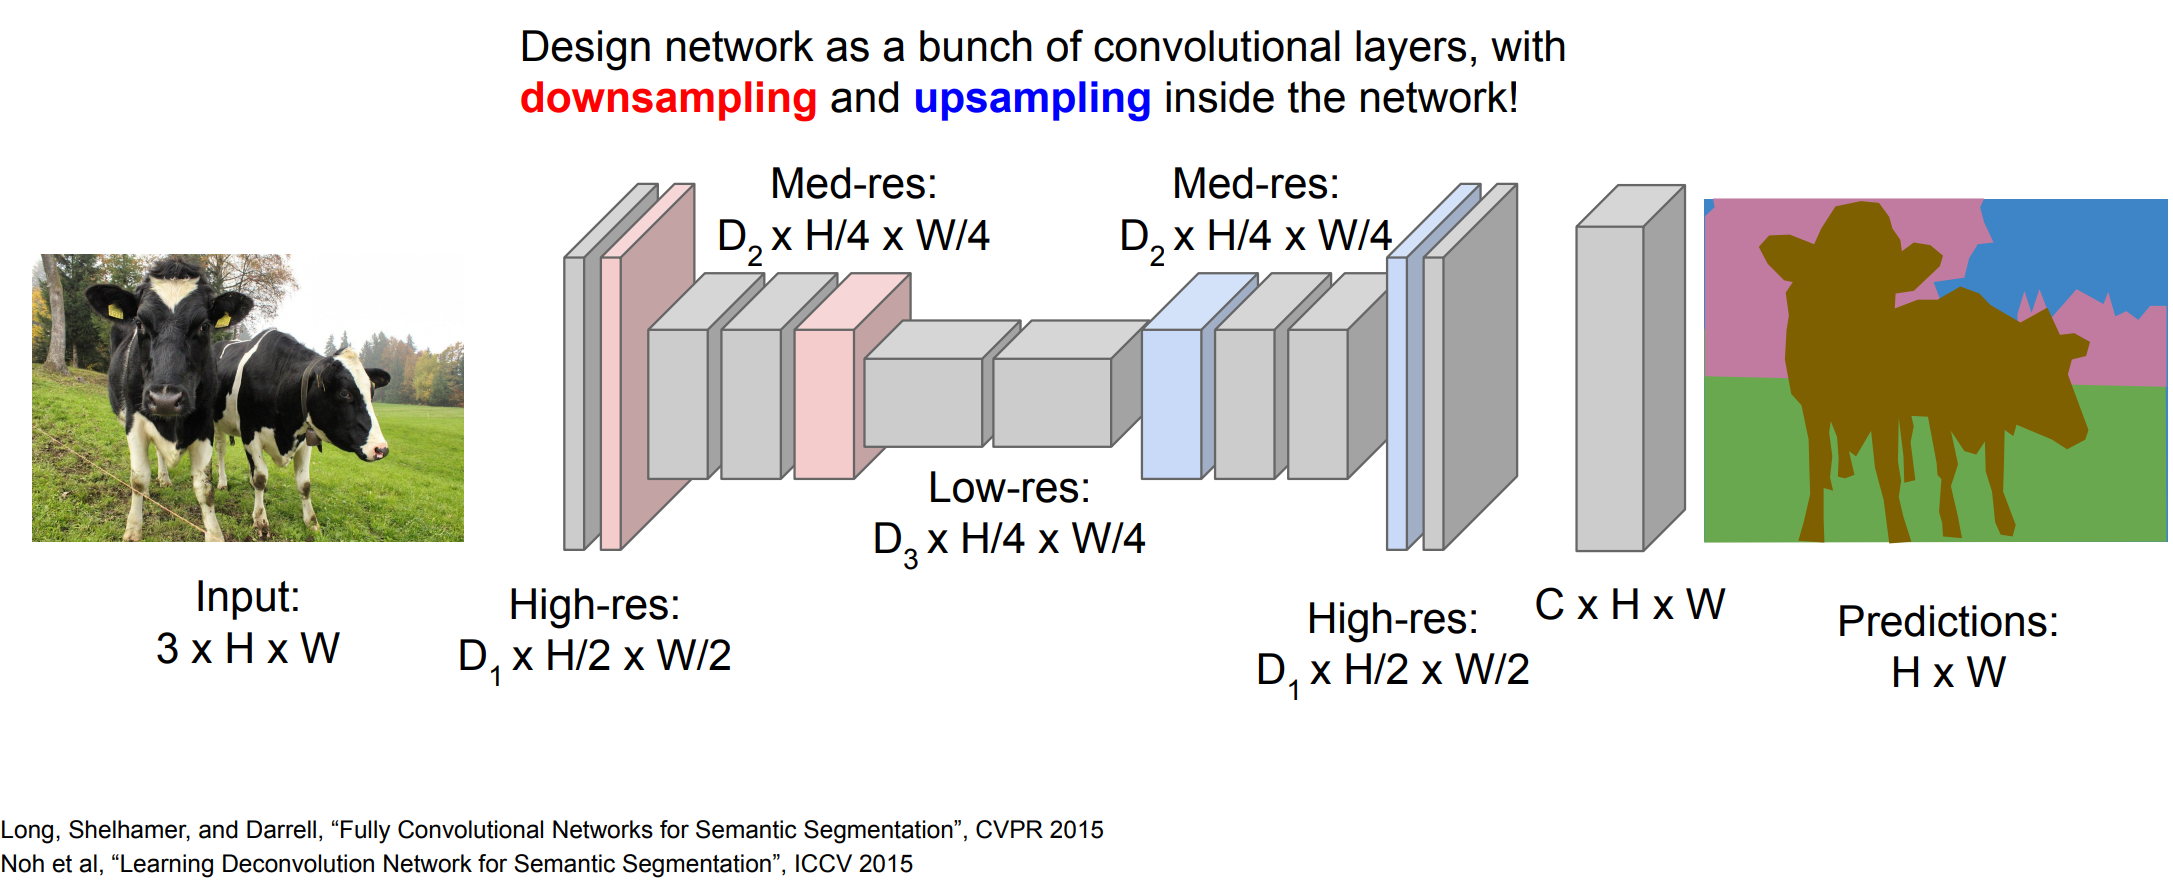
\includegraphics[width=1.0\textwidth,height=1.0\textheight,keepaspectratio]{images/segmentation/sem_9.png}
\end{figure}

\framebreak

\begin{figure}
\centering
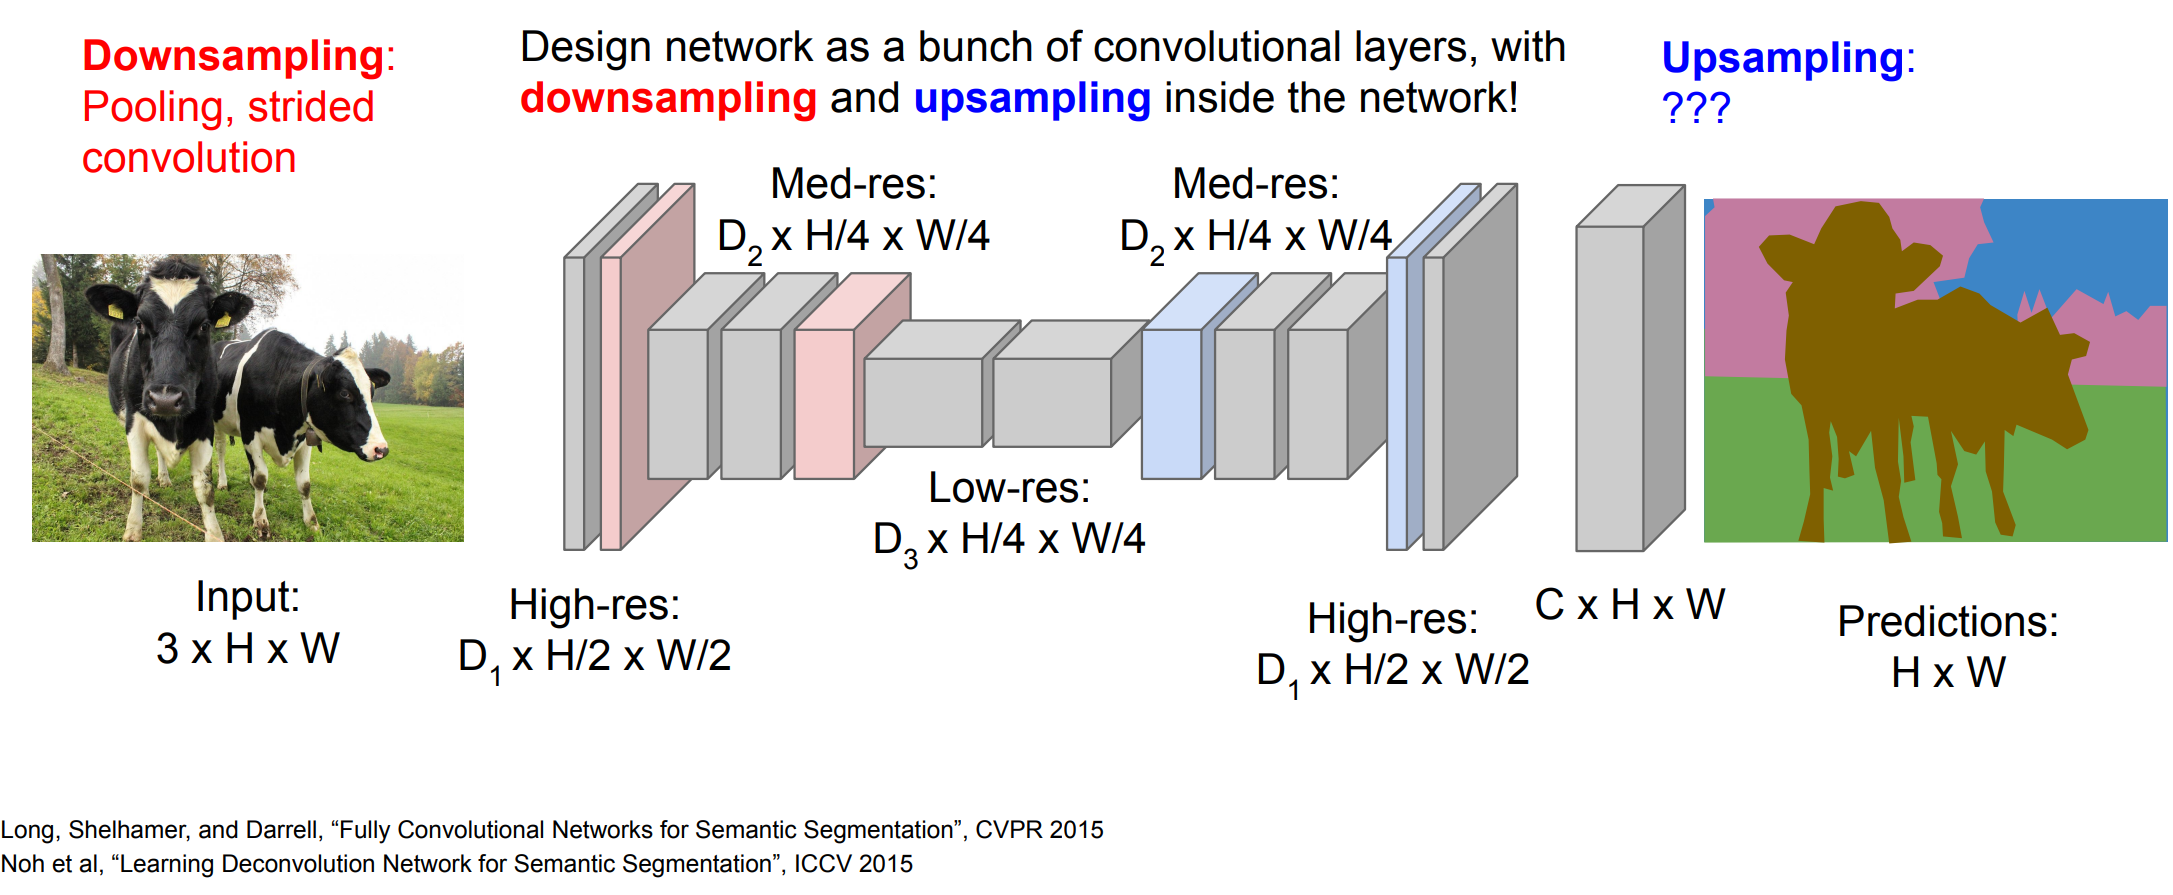
\includegraphics[width=1.0\textwidth,height=1.0\textheight,keepaspectratio]{images/segmentation/sem_10.png}
\end{figure}
    
\end{frame}

